% =====================================================================
%  Tutorial do Bruma
%  Compile com XeLaTeX (ou LuaLaTeX) + BibTeX:
%     xelatex bruma-tutorial && bibtex bruma-tutorial
%     xelatex bruma-tutorial && xelatex bruma-tutorial
%  No Overleaf: Menu → Compiler → XeLaTeX.
%  As figuras ficam em img/ e as referências em bruma.bib.
% =====================================================================
\documentclass[11pt,a4paper]{article}
\usepackage{fontspec}
\usepackage{polyglossia}
\setmainlanguage{portuguese}
\usepackage[a4paper,margin=2.4cm]{geometry}
\usepackage{amsmath,amssymb}
\usepackage{graphicx}
\usepackage{booktabs,tabularx,array}
\usepackage{xcolor}
\usepackage{listings}
\usepackage{tcolorbox}
\usepackage{enumitem}
\usepackage{caption}
\usepackage{microtype}
\usepackage{siunitx}
\sisetup{output-decimal-marker={,}}
\usepackage[numbers,sort&compress]{natbib}
\usepackage[hidelinks]{hyperref}
\usepackage{url}

\definecolor{ciano}{HTML}{0A8F78}
\definecolor{ambar}{HTML}{B26B00}
\definecolor{fundo}{HTML}{F3F7F6}
\hypersetup{colorlinks=true,linkcolor=ciano,citecolor=ciano,urlcolor=ciano}
\lstset{basicstyle=\ttfamily\small,backgroundcolor=\color{fundo},frame=single,rulecolor=\color{black!15},
  columns=fullflexible,breaklines=true,keepspaces=true,showstringspaces=false,
  literate={á}{{\'a}}1 {ã}{{\~a}}1 {é}{{\'e}}1 {ê}{{\^e}}1 {í}{{\'i}}1 {ó}{{\'o}}1 {ç}{{\c c}}1 {ú}{{\'u}}1 {Δ}{{$\Delta$}}1}
\newtcolorbox{nota}[1][]{colback=fundo,colframe=ambar,boxrule=0.6pt,arc=2pt,left=6pt,right=6pt,#1}
\setlist{itemsep=2pt,topsep=4pt}
\graphicspath{{img/}}
\newcommand{\cp}{\textsf{Bruma}}

\title{
\includegraphics[width=0.42\linewidth]{bruma-logo-claro.png}\\[10pt]\textbf{Tutorial do \cp}\\[4pt]\large Estrutura de bandas, DOS, PDOS, densidade de carga, defeitos e termodinâmica\\ a partir de cálculos CASTEP}
\author{Bruno H. D. Macedo\\[2pt]\small Programa de Pós-Graduação em Física Aplicada (PPGFISA), UNILA, Foz do Iguaçu\\
\small \url{https://brunohdmacedo.tech/bruma/} \quad ORCID 0000-0002-8152-0950}
\date{Versão 1.0.0 — novembro de 2026}

\begin{document}
\maketitle
\begin{abstract}
O \cp{} é um software livre (página web, Python para cluster, interface gráfica e programa para Windows) para analisar as saídas do CASTEP~\cite{clark2005castep}:
\begin{itemize}
  \item estrutura de bandas, DOS e PDOS com spin \textit{up} e \textit{down}, sem recalcular a energia de Fermi;
  \item bandas projetadas por orbital;
  \item identificação e distorção local de defeitos pontuais;
  \item energia de formação e termodinâmica de dessorção de hidrogênio;
  \item densidade de carga total e polarizada, em 3D, 2D e em perfis;
  \item contribuição do defeito para a densidade ($\Delta\rho$) e transferência de carga por átomo;
  \item comparação entre vários cálculos.
\end{itemize}
Este tutorial descreve cada etapa, as fórmulas usadas, as boas práticas e como citar o software.
\end{abstract}
\tableofcontents
\newpage

\section{Visão geral}
O \cp{} pode ser usado de quatro formas, que fazem a mesma análise (Tabela~\ref{tab:interfaces}). O princípio central é que \textbf{a energia de Fermi nunca é recalculada}. O valor usado é o que o CASTEP escreveu no \texttt{.bands}, para cada spin; o programa só escolhe o que subtrair do eixo de energia.
\begin{table}[h]\centering\small
\caption{As quatro formas de usar o \cp. Todas têm uma parte ``Sobre'' com autor, links e como citar.}\label{tab:interfaces}
\begin{tabularx}{\linewidth}{lXX}\toprule
Forma & Para quem & Como começar\\\midrule
Página web & análise interativa, sem instalar nada & \url{https://brunohdmacedo.tech/bruma/}\\
Python, linha de comando & cluster e scripts & \texttt{pip install bruma-dft}; \texttt{bruma seed}\\
Python, com janela & uso local com cliques & \texttt{bruma-gui} (Tkinter)\\
Windows & quem não usa Python & instalador \texttt{Bruma-Setup.exe}\\\bottomrule
\end{tabularx}
\end{table}
O nome vem de \textit{bruma}, névoa: a nuvem eletrônica que o programa mostra. As letras também são as iniciais do autor (\textbf{Bru}no \textbf{Ma}cedo). As análises usam NumPy~\cite{harris2020numpy} e Matplotlib~\cite{hunter2007matplotlib}.

\section{Preparação do cálculo no CASTEP}
As palavras-chave abaixo geram todos os arquivos usados pela ferramenta:
\begin{lstlisting}
TASK                    : SPECTRAL           ! ou GeometryOptimization, SinglePoint
SPECTRAL_TASK           : BANDSTRUCTURE      ! DOS para uma malha densa
SPIN_POLARIZED          : TRUE
PDOS_CALCULATE_WEIGHTS  : TRUE               ! .pdos_bin
POPN_CALCULATE          : TRUE               ! Mulliken e ligações
WRITE_FORMATTED_DENSITY : TRUE               ! .den_fmt
\end{lstlisting}
O caminho de bandas é definido no \texttt{.cell}~\cite{setyawan2010}. A DOS quantitativa deve vir de uma malha Monkhorst--Pack densa~\cite{monkhorst1976}. A Tabela~\ref{tab:arquivos} resume os arquivos.
\begin{table}[h]\centering\small
\caption{Arquivos lidos.}\label{tab:arquivos}
\begin{tabularx}{\linewidth}{lX}\toprule
Arquivo & Conteúdo usado\\\midrule
\texttt{seed.bands} & autovalores, $E_F$ por spin, pesos dos k-pontos, célula\\
\texttt{seed.pdos\_bin} & pesos orbitais por banda e k-ponto (PDOS e bandas projetadas)\\
\texttt{seed.castep} & camadas e orbitais $m$, Mulliken~\cite{mulliken1955,segall1996}, ligações, energias, forças, $Z$ de valência\\
\texttt{seed.cell} & espécies, estrutura do defeito, base para as referências\\
\texttt{.den\_fmt}, \texttt{.cube}, \texttt{CHGCAR} & densidade de carga e de spin\\\bottomrule
\end{tabularx}
\end{table}

\section{Estrutura eletrônica}
\subsection{Bandas, DOS e PDOS}
\begin{itemize}
  \item \textbf{Bandas:} spin \textit{up} e \textit{down} sobrepostos, lado a lado ou separados, com os rótulos de alta simetria detectados automaticamente.
  \item \textbf{DOS:} soma de gaussianas de largura $\sigma$.
  \item \textbf{PDOS:} por elemento, por orbital $l$, por camada $(n,l)$ do pseudopotencial (por exemplo Mg~2p e 3p), por componente $m$, por $t_{2g}/e_g$ ou por átomo.
  \item \textbf{Bandas projetadas:} o tamanho de cada ponto é proporcional ao peso do orbital.
\end{itemize}
\begin{equation}
g_s(E)=\sum_k w_k\sum_n \frac{1}{\sigma\sqrt{2\pi}}\,e^{-(E-\varepsilon_{nks})^2/2\sigma^2},\qquad
g^{\alpha}_s(E)=\sum_k w_k\sum_n p^{\alpha}_{nks}\,\delta_\sigma(E-\varepsilon_{nks}).
\end{equation}
\begin{figure}[h]\centering
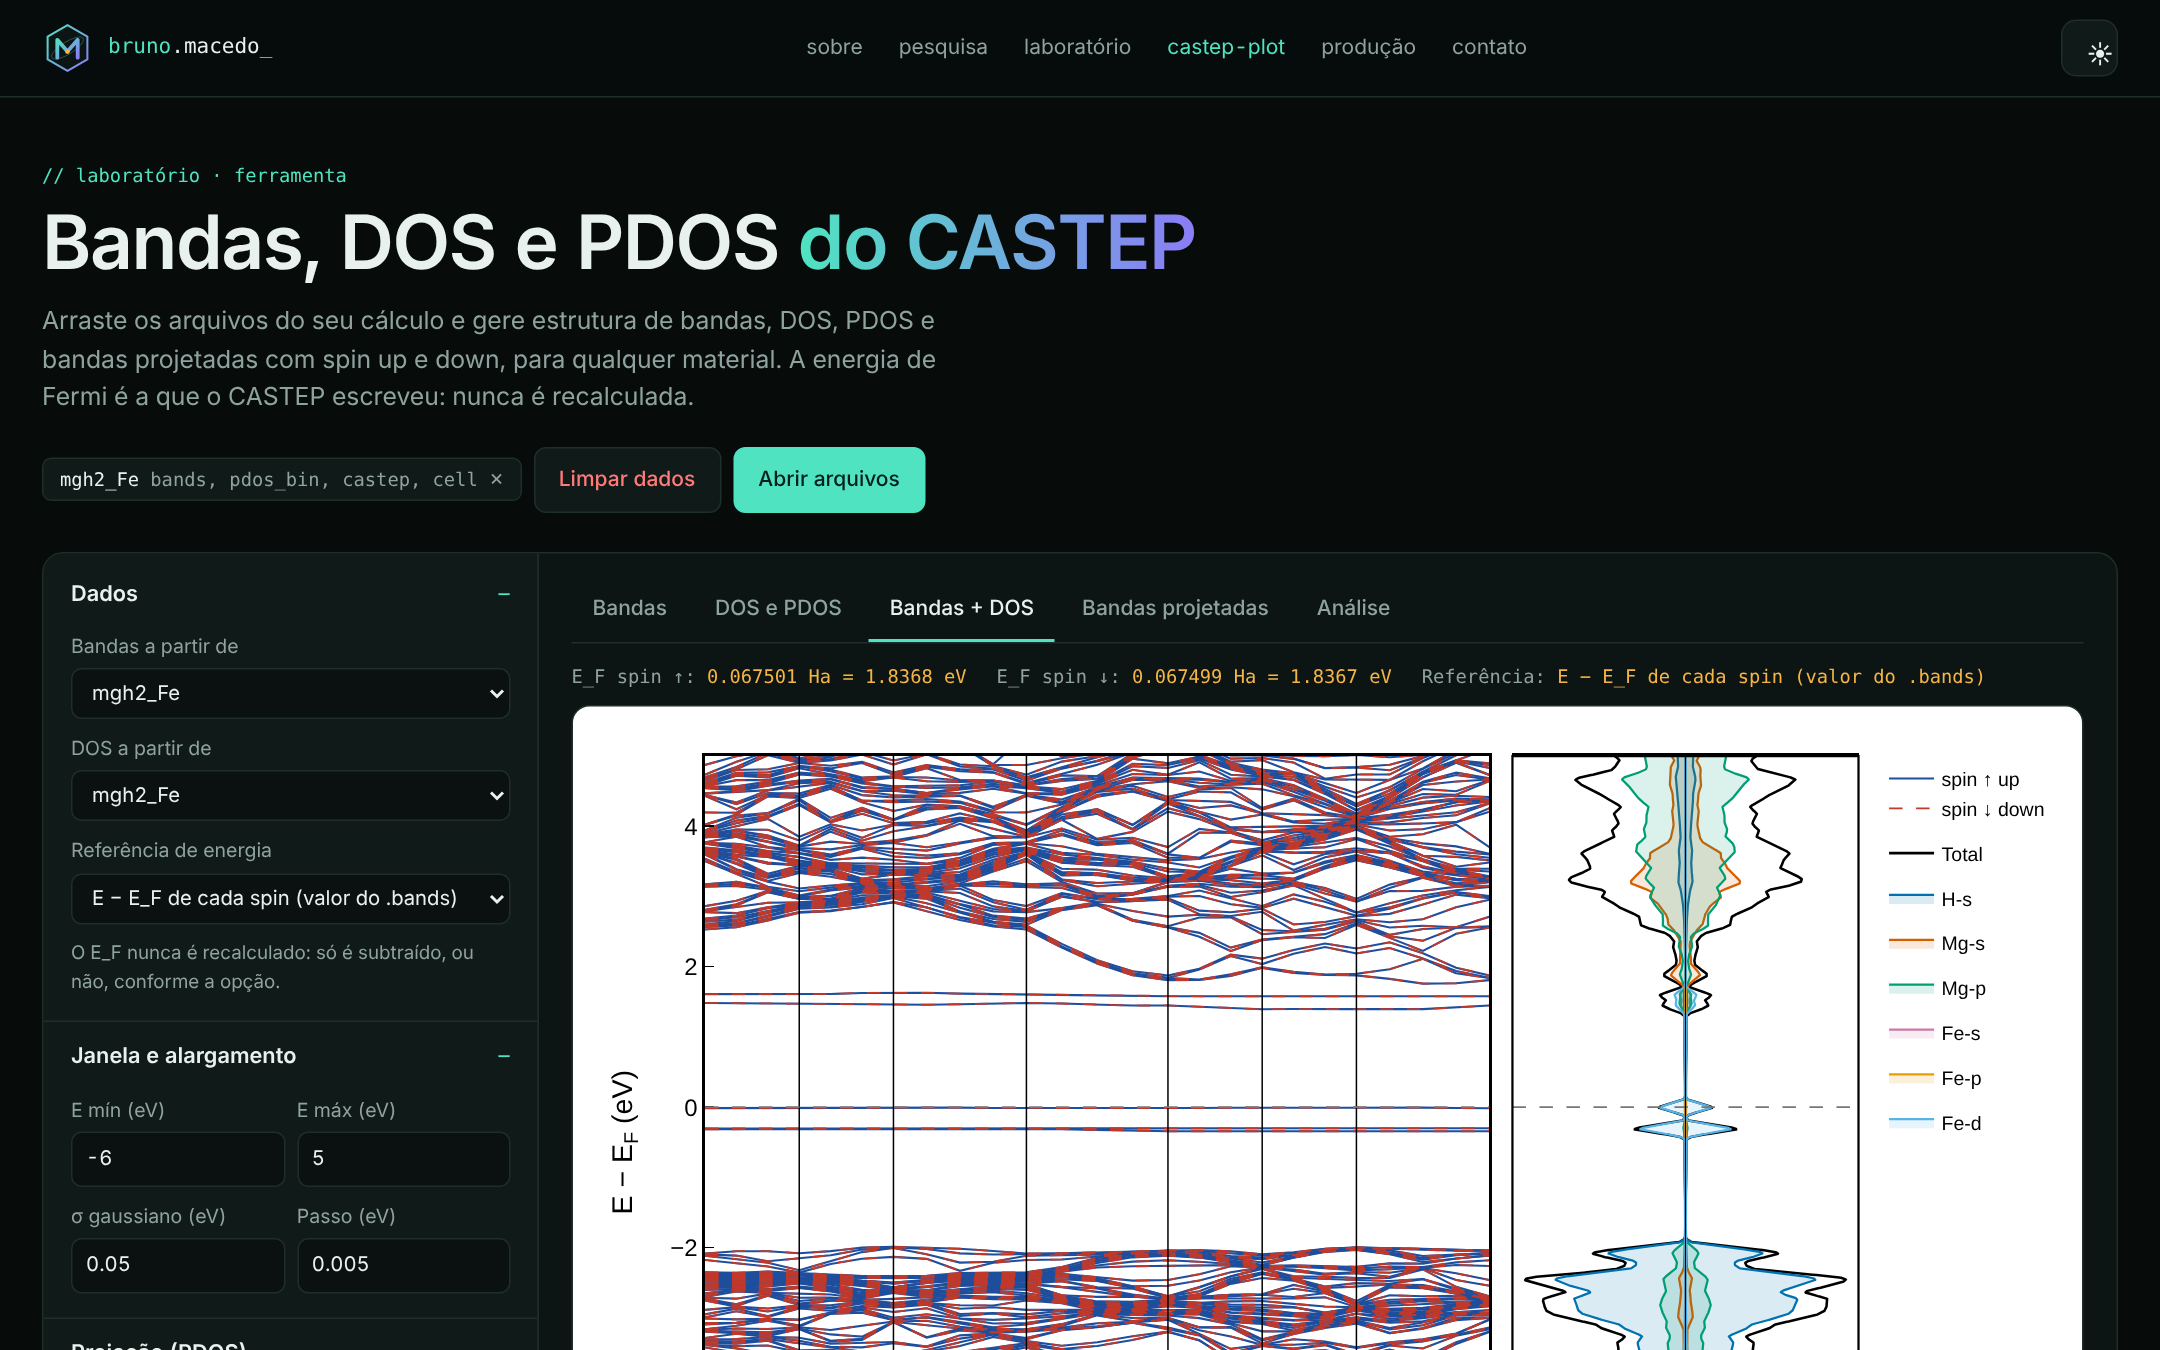
\includegraphics[width=0.92\linewidth]{site_bandas_dos.png}
\caption{Bandas e DOS de MgH$_2$:Fe no site.}
\end{figure}

\subsection{Análise}
O gap é definido pela contagem de elétrons, com $N$ elétrons por spin:
\begin{equation}
E_g=\min_k\varepsilon_{N+1,k}-\max_k\varepsilon_{N,k}.
\end{equation}
Isso evita que uma banda quase plana no nível de Fermi seja lida como gap nulo. A ferramenta informa ainda:
\begin{itemize}
  \item o $E_F$ por spin e se ele cai dentro de alguma banda;
  \item a polarização em $E_F$, $P=(N_\uparrow-N_\downarrow)/(N_\uparrow+N_\downarrow)$;
  \item as ocupações integradas da PDOS e o centro da banda d;
  \item as cargas e spins de Mulliken.
\end{itemize}

\section{Defeitos e distorção da estrutura}
Com a estrutura pura de referência, cada átomo é casado com o seu sítio, com condições periódicas, e o tipo de defeito (vacância, substitucional ou intersticial) é identificado sozinho. Sem referência, o entorno do defeito é comparado com o \textit{bulk} da própria supercélula.

São calculados os primeiros vizinhos, as ligações dos vizinhos (por exemplo H--Mg), a segunda camada e os índices de distorção do poliedro:
\begin{equation}
D=\frac1n\sum_i\frac{|d_i-\bar d|}{\bar d},\quad
\langle\lambda\rangle=\frac1n\sum_i\Big(\frac{d_i}{l_0}\Big)^{2},\quad
\sigma^2=\frac{1}{m-1}\sum_j(\theta_j-\theta_0)^2,\quad
\mathrm{ECoN}=\sum_i e^{\,1-(d_i/d_{\mathrm{av}})^6},
\end{equation}
\begin{itemize}
  \item $D$ é o índice de Baur~\cite{baur1974};
  \item $\langle\lambda\rangle$ e $\sigma^2$ seguem Robinson, Gibbs e Ribbe~\cite{robinson1971}, com $l_0$ a distância centro--vértice do poliedro regular de mesmo volume;
  \item ECoN é a coordenação efetiva de Hoppe~\cite{hoppe1979}.
\end{itemize}
Com a referência, também são calculados o campo de deslocamentos $|\Delta\mathbf r|$ em função da distância ao defeito, o raio de perturbação e $\Delta V/V$.

\section{Termodinâmica}
Com $\mu_i$ a energia por átomo das referências elementares e $\mu_\mathrm{H}=\tfrac12E(\mathrm{H}_2)$~\cite{freysoldt2014,vandewalle2004}:
\begin{align}
E_f&=E_\mathrm{def}-E_\mathrm{pura}-\sum_i n_i\mu_i, &
\Delta H_f&=\frac{E-\sum_i N_i\mu_i}{N_\mathrm{H}/2}, &
T_d&=\frac{\Delta H}{\Delta S}.
\end{align}
O $\Delta H_f$ é dado em kJ/mol de H$_2$. Para $T_d$ usa-se $\Delta S\approx\SI{130.7}{J\,mol^{-1}K^{-1}}$, a entropia padrão do H$_2$~\cite{chase1998janaf}, uma aproximação comum para hidretos~\cite{sakintuna2007}. A ferramenta calcula ainda o efeito do defeito $\Delta\Delta H=\Delta H_\mathrm{def}-\Delta H_\mathrm{pura}$, a energia de remoção de H e a capacidade gravimétrica.

\begin{nota}
As energias são eletrônicas a \SI{0}{K}, sem energia de ponto zero. Compare apenas cálculos com o mesmo funcional (por exemplo PBE~\cite{perdew1996pbe}), corte, pseudopotenciais e U de Hubbard.
\end{nota}

\subsection{Geração dos cálculos de referência}
A partir do \texttt{.cell} do defeito, a ferramenta gera \texttt{.cell} e \texttt{.param} com os mesmos parâmetros do cálculo original (Tabela~\ref{tab:refs}).
\begin{table}[h]\centering\small
\caption{Cálculos de referência gerados.}\label{tab:refs}
\begin{tabularx}{\linewidth}{lX}\toprule
Cálculo & Uso\\\midrule
\texttt{seed\_puro} & estrutura pura (relaxada)\\
\texttt{seed\_dif\_puro\_fixo} & hospedeiro na geometria do defeito (\textit{single point}): $\Delta\rho$ sem dipolos de relaxação\\
\texttt{seed\_dif\_sem\_X}, \texttt{seed\_dif\_so\_X} & densidade de ligação do dopante\\
\texttt{seed\_semH\_perto/longe} & energia de remoção de H perto e longe do defeito\\
\texttt{Mg\_hcp}, \texttt{Fe\_bcc}, \texttt{H\_H2}, \ldots & potenciais químicos\\\bottomrule
\end{tabularx}
\end{table}

\section{Densidade de carga}
\subsection{Grandezas, cargas e exportação}
As grandezas disponíveis são $\rho$, $\rho_\uparrow$, $\rho_\downarrow$, $\rho_\uparrow-\rho_\downarrow$, $|\rho_\uparrow-\rho_\downarrow|$, $\zeta=(\rho_\uparrow-\rho_\downarrow)/\rho$ e $\Delta\rho$. Elas podem ser vistas como isosuperfície 3D, em cortes 2D e em perfis ao longo de ligações. O mínimo do perfil aproxima o ponto crítico de ligação.

\textbf{Cargas e momentos por átomo.} São obtidos por partição de Voronoi~\cite{voronoi1908}. Na versão radical~\cite{gellatly1982}, cada ponto vai para o átomo que minimiza $|\mathbf r-\mathbf R_a|^2-r_a^2$, com os raios covalentes de Cordero~\cite{cordero2008}.

\textbf{Exportação.} A densidade pode ser exportada como CHGCAR (formato VASP 5 com os elementos, em $\rho V$) ou XSF, para o VESTA~\cite{momma2011vesta} e o programa \texttt{bader}~\cite{henkelman2006}. Também são lidos arquivos \texttt{.cube}, como os do \texttt{c2x}~\cite{rutter2018c2x}.

\subsection{Planos cristalográficos}
\begin{itemize}
  \item A multiplicidade da supercélula é detectada sozinha (por exemplo $3\times3\times3$ do rutilo), e os índices $(hkl)$ são os do material.
  \item Os eixos do corte seguem direções da rede contidas no plano; no (110), [$\bar1$10] e [001].
  \item O corte cobre a seção inteira da supercélula e pode ser deslocado ao longo da normal.
  \item Uma galeria mostra os planos principais lado a lado.
\end{itemize}
\begin{figure}[h]\centering
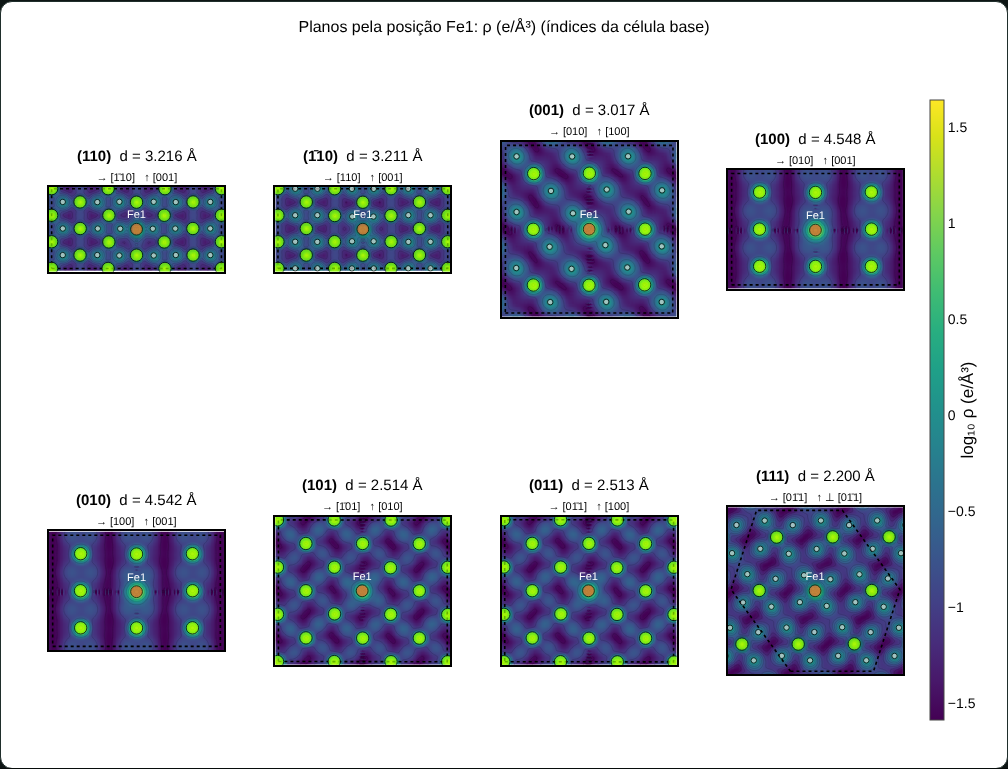
\includegraphics[width=0.95\linewidth]{site_galeria_planos.png}
\caption{Galeria de planos pelo dopante.}
\end{figure}

\subsection{Contribuição do defeito}
Há três formas de isolar o efeito do defeito na densidade:
\begin{enumerate}
  \item $\rho_\mathrm{def}-\rho_\mathrm{pura}$: inclui a relaxação.
  \item $\rho_\mathrm{def}-\rho_\mathrm{pura}^{\,\mathrm{geometria\ do\ defeito}}$: mesma grade e mesmas posições.
  \item $\rho_\mathrm{def}-\rho_\mathrm{sem\ X}-\rho_\mathrm{s\acute{o}\ X}$: densidade de ligação.
\end{enumerate}
A diferença é feita componente a componente:
\begin{equation}
\Delta\rho=\pm(\rho_\mathrm{def}-\rho_\mathrm{pura}),\quad
\Delta\rho_\uparrow,\quad \Delta\rho_\downarrow,\quad \Delta(\rho_\uparrow-\rho_\downarrow),
\end{equation}
no sentido escolhido: defeito $-$ puro ou puro $-$ defeito. A diferença pode ser vista em 3D (isosuperfícies $\pm$, na célula inteira ou numa caixa de $\pm3$ a $\pm6$\,\AA{} em volta do dopante) e em 2D, nos planos $(hkl)$. Na aba Comparação, as diferenças de todos os defeitos aparecem lado a lado em 3D e 2D. Um pacote \texttt{.zip} para o VESTA~\cite{momma2011vesta} traz, para cada estrutura, os CHGCARs de $\rho$, $\rho_\uparrow$, $\rho_\downarrow$, $\rho_\uparrow-\rho_\downarrow$ e das quatro diferenças, com um guia de visualização. Se as grades diferirem, a densidade subtraída é reamostrada por interpolação trilinear. A ferramenta informa os elétrons ganhos e perdidos, as integrais em esferas e a transferência de carga por átomo, $\int_{V_a}\Delta\rho\,dV$.

\begin{figure}[h]\centering
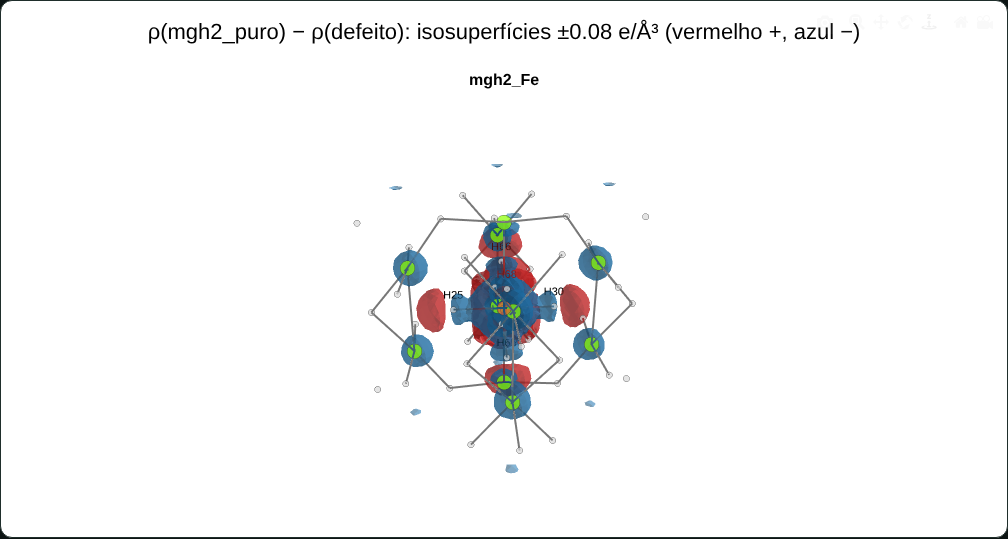
\includegraphics[width=0.8\linewidth]{site_delta_rho_3d.png}
\caption{$\rho_\mathrm{pura}-\rho_\mathrm{def}$ em 3D numa caixa de $\pm4$\,\AA{} em volta do dopante (vermelho $+$, azul $-$; densidade de teste).}
\end{figure}

\subsection{Relatório da diferença de densidade}
Uma aba dedicada reúne as grandezas que descrevem a redistribuição de carga:
\begin{equation}
Q_\pm=\int_{\Delta\rho\gtrless0}\Delta\rho\,dV,\qquad
Q_\mathrm{red}=\tfrac12\int|\Delta\rho|\,dV,\qquad
\mathbf p=\int(\mathbf r-\mathbf r_c)\,\Delta\rho\,dV,\qquad
\Delta Q(r)=\int_0^r\overline{\Delta\rho}(r')\,4\pi r'^2\,dr'.
\end{equation}
A aba mostra ainda:
\begin{itemize}
  \item os raios que contêm 50\,\% e 90\,\% de $Q_\mathrm{red}$;
  \item os pontos de máximo acúmulo e depleção;
  \item as médias planares ao longo de $a$, $b$ e $c$;
  \item o $\rho$ mínimo de cada ligação dopante--vizinho contra a mesma ligação do hospedeiro no puro;
  \item a carga de Voronoi de cada átomo nas duas estruturas, casadas pelo mapeamento;
  \item os trípticos $\rho_\mathrm{pura}$ | $\rho_\mathrm{def}$ | $\Delta\rho$ em 2D e 3D.
\end{itemize}
O dipolo só independe da origem quando $\Delta N=0$.

\section{Comparação entre cálculos}
A aba Comparação monta uma tabela com uma coluna por cálculo, exportável em \texttt{.dat} para o Origin. Ela reúne energias, $E_f$, $\Delta H$, $T_d$, gaps, $N(E_F)$, polarização, PDOS d, cargas, distorções e parâmetros de célula. Também gera gráficos: barras, DOS e PDOS sobrepostas, bandas lado a lado, ligações, deslocamentos e densidade (inclusive $\Delta\rho$) no mesmo plano.
\begin{figure}[h]\centering
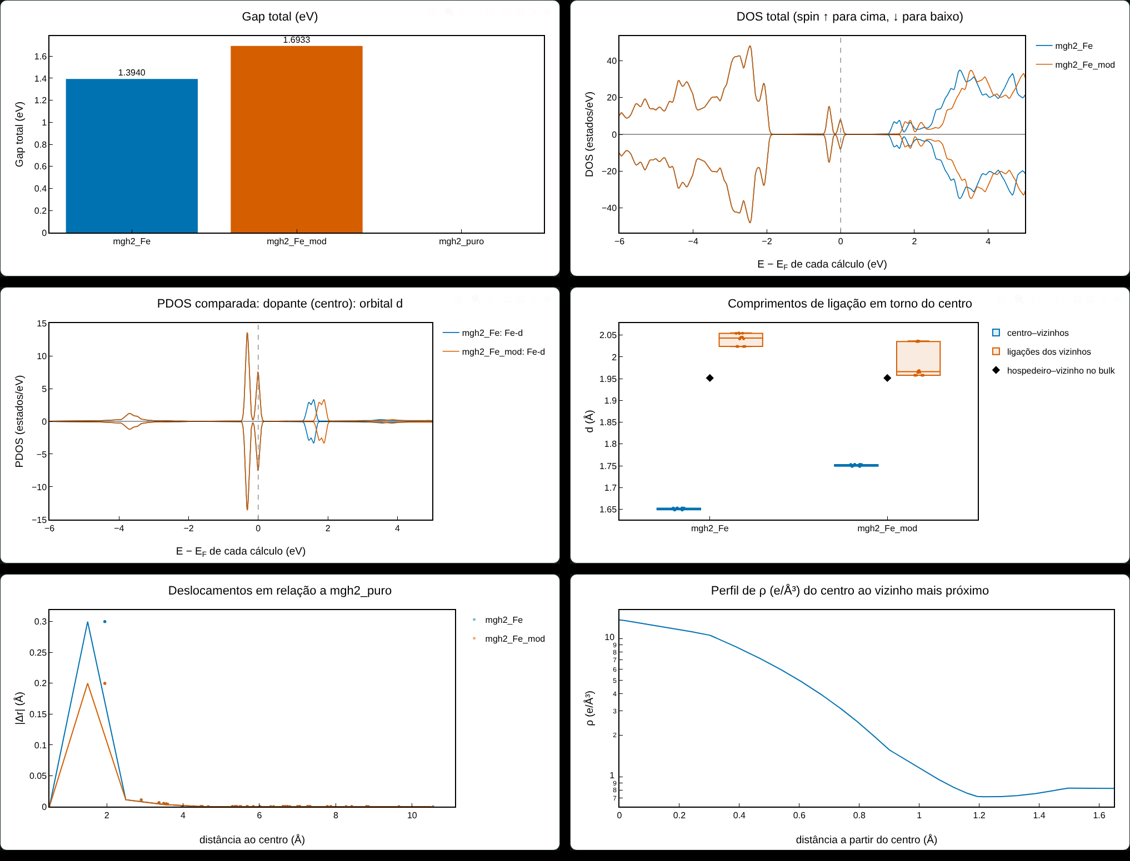
\includegraphics[width=0.95\linewidth]{site_comparacao.png}
\caption{Gráficos da aba Comparação (exemplo ilustrativo).}
\end{figure}

\section{Script Python}
\begin{lstlisting}
python3 bruma.py mgh2_Fe -e Mg,H,Fe
python3 bruma.py mgh2_Fe --ref mgh2_puro --mu "Mg=@Mg_hcp,Fe=@Fe_bcc,H=@H_H2"
python3 bruma.py mgh2_Fe --gerar-referencias
python3 bruma.py mgh2_Fe --planes todos --field spin --chgcar
python3 bruma.py mgh2_Fe --field diff --subtract mgh2_Fe_dif_puro_fixo.den_fmt
python3 bruma.py mgh2_Fe --vesta --subtract mgh2_puro.den_fmt --diff-sign puro-defeito
\end{lstlisting}

\section{Cuidados e limitações}
\begin{itemize}
  \item A DOS do caminho de bandas é ilustrativa.
  \item O gap e as bordas vêm só dos k-pontos do caminho.
  \item As componentes $m$ estão nos eixos cartesianos da célula.
  \item As cargas de Voronoi são estimativas; para números quantitativos, use Bader.
  \item $\Delta\rho$ com grades diferentes é reamostrado.
\end{itemize}

\section{Como citar}
Ao usar o \cp, cite o software~\cite{macedo2026bruma} e o CASTEP~\cite{clark2005castep}. Quando fizer sentido, cite também o TCC~\cite{macedo2025tcc} e a dissertação~\cite{macedo2027dissertacao} do autor, que motivaram o desenvolvimento, o trabalho apresentado no 2º Encontro de Física Aplicada na Tríplice Fronteira~\cite{macedo2025efatf} e, em aplicações de aprendizado de máquina, o artigo~\cite{macedo2024rbic} e a base de dados de exoplanetas~\cite{macedo2024dataset}. Os registros estão em \texttt{bruma.bib} e no \texttt{CITATION.cff} do repositório.

\begin{nota}[title={Referência sugerida (ABNT)}]
MACEDO, B. H. D. \textbf{Bruma}: análise de estrutura de bandas, DOS, PDOS, densidade de carga, defeitos e termodinâmica de cálculos CASTEP. Versão 1.0. Foz do Iguaçu, 2026. Software. Disponível em: \url{https://brunohdmacedo.tech/bruma/}. Acesso em: [data].
\end{nota}

\nocite{ganose2018sumo,plotly2015}
\bibliographystyle{unsrtnat}
\bibliography{Bruma}
\end{document}
